\section{Apprendimento non supervisionato}
\label{app_non_sup}

Nel capitolo precedente è stata mostrata l'utilità degli algoritmi di apprendimento supervisionato, osservando che, nel caso in cui si abbiano a disposizione sia i vettori di input che i corrispettivi output target, si può ottenere un'approssimazione della relazione esistente input-output.
Tuttavia non è sempre possibile avere a disposizione gli output target e bisogna capire se è comunque possibile ottenere informazioni utili dai dati. \\
Come già accennato nelle prime pagine di questa trattazione quando non si hanno a disposizione gli output target si possono applicare tecniche di apprendimento non supervisionato, dove l'obiettivo è quello di trovare eventuali partizioni degli input (Clustering). \\
Si consideri la figura ~\ref{Unsup} dove sono riportate tre diverse configurazioni possibili nel caso di input bidimensionali: è evidente che nel caso a) sia possibile la separazione in due sotto gruppo e nel caso b) in un unico sotto gruppo, mentre nel caso c) sembrerebbe non si possano stabilire graficamente eventuali separazioni.

\begin{figure}[h!]
	\centering
	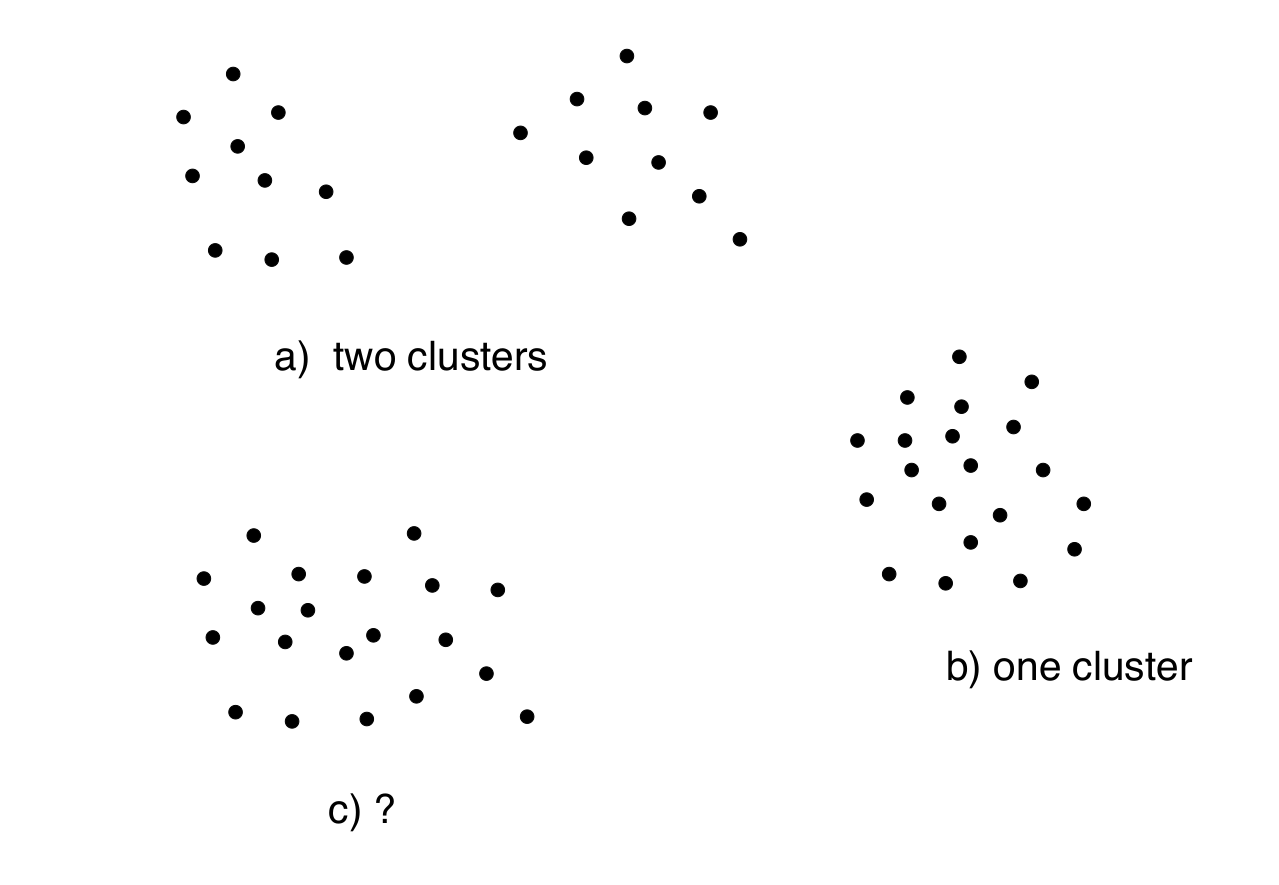
\includegraphics[width=0.85\textwidth]{figs/Unsup_learning.png}
	\caption{vettori di input in uno spazio bidimensionale in tre situazioni differenti. L'immagine è presa da \cite{IntroML}}
	\label{Unsup}
\end{figure}

Quindi un algoritmo di clustering si occupa della suddivisione del set di input $\Sigma$ in un numero N di sottogruppi $\Sigma_1$,...,$\Sigma_n$, detti appunto cluster; si noti che lo stesso numero N non viene stabilito a priori e fornito all'algoritmo, ma viene anch'esso ricavato a partire dai dati. Una volta fatto sarà possibile implementare un classificatore per collegare nuovi vettori di input con i cluster precedentemente individuati.\\
Inoltre, aumentando il livello di complessità, è possibile trovare eventuali gerarchie di partizionamento, ovvero cluster di cluster.


\newpage